\section{Thực nghiệm}
\subsection{Miêu tả bộ dữ liệu}
\subsubsection{Giới thiệu bộ dữ liệu sử dụng}

MOOCCubeX là một trong những bộ dữ liệu lớn nhất và chi tiết nhất về MOOCs (Massive Open Online Courses), hỗ trợ các nghiên cứu về hành vi học tập trực tuyến và cá nhân hóa học tập. Bộ dữ liệu được xây dựng bởi Nhóm Kỹ thuật Tri thức (Knowledge Engineering Group) tại Đại học Thanh Hoa (Tsinghua University), Trung Quốc, với sự hợp tác của XuetangX, một nền tảng MOOC lớn tại Trung Quốc. Đây là bộ dữ liệu đa dạng, phục vụ cho nghiên cứu trong các lĩnh vực như học máy, hệ thống học tập thích ứng, phân tích giáo dục, và trí tuệ nhân tạo.

MOOCCubeX bao gồm nhiều loại dữ liệu khác nhau, tập trung vào các khóa học và hành vi học tập của học viên. Các thành phần chính của bộ dữ liệu bao gồm:

\begin{itemize}
    \item \textbf{Courses:}
    \begin{itemize}
        \item Số lượng khóa học: 4,216.
        \item Nội dung: Mỗi khóa học bao gồm các video giảng dạy, bài tập, và bài kiểm tra. Thông tin về mỗi khóa học bao gồm tiêu đề, mô tả, người hướng dẫn, ngày bắt đầu và ngày kết thúc, ngôn ngữ giảng dạy và lĩnh vực học tập.
    \end{itemize}

    \item \textbf{Video:}
    \begin{itemize}
        \item Số lượng: 230,263.
        \item Thông tin: Các video giảng dạy được thu thập từ các khóa học trên nền tảng MOOC. Mỗi video có các thuộc tính như tiêu đề, thời lượng, nội dung được giảng dạy, và số lần xem của học viên.
    \end{itemize}

    \item \textbf{Exercise:}
    \begin{itemize}
        \item Số lượng: 258,265.
        \item Thông tin: Bao gồm các bài tập tự luyện và kiểm tra đánh giá. Các bài tập này được thiết kế để giúp học viên ôn luyện kiến thức và kiểm tra khả năng tiếp thu sau mỗi phần học.
    \end{itemize}

    \item \textbf{Problem:}
    \begin{itemize}
        \item Số lượng: 2,454,397 vấn đề.
        \item Thông tin: Thường là các vấn đề hoặc câu hỏi phức tạp yêu cầu học viên giải quyết bằng cách áp dụng kiến thức học được từ khóa học.
    \end{itemize}

    \item \textbf{Student Profile:}
    \begin{itemize}
        \item Số lượng: 3,330,294 hồ sơ.
        \item Thông tin: Hồ sơ học viên lưu trữ các thông tin về hành vi học tập, tiến trình học tập và các hoạt động của họ trên nền tảng.
    \end{itemize}

    \item \textbf{Video Watching Behavior:}
    \begin{itemize}
        \item Số lượng: 154,332,174 dữ liệu.
        \item Thông tin: Dữ liệu hành vi xem video cung cấp thông tin chi tiết về cách học viên tương tác với video giảng dạy. Dữ liệu này giúp nghiên cứu thói quen học tập của học viên.
    \end{itemize}

    \item \textbf{Comment and Reply:}
    \begin{itemize}
        \item Số lượng: 8,422,134 bản ghi phản hồi bình luận.
        \item Thông tin: Bình luận và phản hồi là phần quan trọng trong việc đánh giá mức độ tương tác của học viên với khóa học. Là cơ sở để phân tích cảm xúc của học viên, đánh giá mức độ hài lòng và tìm kiếm những khó khăn mà học viên gặp phải trong quá trình học.
    \end{itemize}
\end{itemize}

Bộ dữ liệu MOOCCubeX được cung cấp dưới dạng các tệp tin JSON và CSV, cho phép người dùng dễ dàng tải xuống và sử dụng. Đây là một bộ dữ liệu quý giá cho nghiên cứu về giáo dục trực tuyến và học tập thích ứng. Với khối lượng dữ liệu lớn và đa dạng, bộ dữ liệu này mở ra nhiều cơ hội cho các nhà nghiên cứu trong việc hiểu sâu hơn về hành vi học tập và xây dựng các hệ thống học tập tiên tiến, giúp cải thiện hiệu quả giáo dục trên các nền tảng trực tuyến.

\subsubsection{Mô tả về tập dữ liệu}

\textbf{I. Courses}

Phần này mô tả về khóa học (course) và các tài nguyên liên quan, bao gồm các file: \texttt{course.json}, \texttt{video.json}, \texttt{problem.json}, \texttt{school.json}, \texttt{teacher.json}, \texttt{course-field.json}, \texttt{course-school.txt}, \texttt{course-teacher.txt}, \texttt{exercise-problem.txt}, và \texttt{video\_id-ccid.txt}.

Dưới đây là bảng sơ lược về các file:

\begin{table}[H]
\centering
\resizebox{\textwidth}{!}{%
\begin{tabular}{|l|l|p{7cm}|l|}
\hline
\textbf{Tên} & \textbf{Loại} & \textbf{Mô tả} & \textbf{Kích thước} \\ \hline
\texttt{course.json} & entities & Tổ chức video và bài tập của khóa học. & 43MB \\ \hline
\texttt{video.json} & entities & Tên video và phụ đề. & 580MB \\ \hline
\texttt{exercise-problem.txt} & relations & Một nhóm các bài tập của khóa học. & 129MB \\ \hline
\texttt{problem.json} & entities & Các bài tập thực hành trong một nhóm bài tập. & 1.2GB \\ \hline
\texttt{school.json} & entities & Thông tin về trường học. & 613KB \\ \hline
\texttt{teacher.json} & entities & Thông tin về giáo viên. & 8.7MB \\ \hline
\texttt{course-field.json} & relations & Lĩnh vực mà khóa học thuộc về, được chú thích bởi con người. & 62KB \\ \hline
\end{tabular}%
}
\caption{Bảng mô tả các file trong tập dữ liệu Courses}
\end{table}

\textbf{Bảng \texttt{course.json}}

\begin{table}[H]
\centering
\resizebox{\textwidth}{!}{%
\begin{tabular}{|l|p{7cm}|l|l|}
\hline
\textbf{Thuộc tính} & \textbf{Nội dung} & \textbf{Kiểu dữ liệu} & \textbf{Miền giá trị} \\ \hline
about & Giới thiệu khóa học & string & \\ \hline
id & ID của khóa học & string & Bắt đầu bằng \texttt{"C\_"} \\ \hline
field & Danh sách các lĩnh vực của khóa học & list<string> & \\ \hline
name & Tên trường & string & \\ \hline
prerequisites & Nội dung về kiến thức tiên quyết & string & \\ \hline
resource & Danh sách các tài nguyên & list<Resource> & \\ \hline
\end{tabular}%
}
\caption{Cấu trúc bảng \texttt{course.json}}
\end{table}

\textbf{Bảng Resource}

\begin{table}[H]
\centering
\resizebox{\textwidth}{!}{%
\begin{tabular}{|l|p{7cm}|l|l|}
\hline
\textbf{Thuộc tính} & \textbf{Nội dung} & \textbf{Kiểu dữ liệu} & \textbf{Miền giá trị} \\ \hline
resource\_id & ID của tài nguyên & string & Bắt đầu bằng \texttt{"V\_"} nếu là video, \texttt{"Ex\_"} nếu là bài tập. \\ \hline
chapter & Số chương & list<string> & \\ \hline
titles & Danh sách các tiêu đề (chương, video, ...) & list<string> & Có tối đa 3 cấp tiêu đề \\ \hline
\end{tabular}%
}
\caption{Cấu trúc bảng Resource}
\end{table}

\textbf{Bảng \texttt{video.json}}

\begin{table}[H]
\centering
\resizebox{\textwidth}{!}{%
\begin{tabular}{|l|p{7cm}|l|l|}
\hline
\textbf{Thuộc tính} & \textbf{Nội dung} & \textbf{Kiểu dữ liệu} & \textbf{Miền giá trị} \\ \hline
ccid & ID duy nhất của video & string & \\ \hline
name & Tên của video & string & \\ \hline
start & Thời gian bắt đầu của từng câu trong phụ đề video & list<float> & \\ \hline
end & Thời gian kết thúc của từng câu trong phụ đề video & list<float> & \\ \hline
text & Phụ đề của từng câu trong video & list<string> & \\ \hline
\end{tabular}%
}
\caption{Cấu trúc bảng \texttt{video.json}}
\end{table}

\textbf{Các bảng khác:}

\begin{itemize}
    \item \textbf{\texttt{exercise-problem.json}}: Dữ liệu bài tập, định dạng: \texttt{exercise ID\t question ID}, kích thước: 129MB.
    \item \textbf{\texttt{problem.json}}:
    \begin{itemize}
        \item \textbf{Thuộc tính:} ID, exercise\_id, language, title, content, option, answer, score, type, typetext, location, context\_id.
        \item \textbf{Kích thước:} 1.2GB.
    \end{itemize}
    \item \textbf{\texttt{school.json}}: Thông tin trường học.
    \item \textbf{\texttt{teacher.json}}: Thông tin giáo viên.
    \item \textbf{\texttt{course-field.json}}: Liên kết lĩnh vực với khóa học.
\end{itemize}
\textbf{II. User}

Phần này mô tả hành vi người học (\textit{user}), bao gồm các file: \texttt{user.json}, \texttt{comment.json}, \texttt{reply.json}, \texttt{course-comment.txt}, \texttt{user-comment.txt}, \texttt{user-reply.txt}, \texttt{comment-reply.txt}, \texttt{user-problem.json}, \texttt{user-video.json}, và \texttt{user-xiaomu.json}.

\textbf{Bảng sơ lược về các file:}

\begin{table}[H]
\centering
\resizebox{\textwidth}{!}{%
\begin{tabular}{|l|l|p{7cm}|l|}
\hline
\textbf{Tên} & \textbf{Loại} & \textbf{Mô tả} & \textbf{Kích thước} \\ \hline
\texttt{user.json} & entities & Thông tin của học sinh (user) & 770MB \\ \hline
\texttt{comment.json} & entities & Thông tin bình luận của user lên từng tài nguyên của course & 2.1GB \\ \hline
\texttt{reply.json} & entities & Thông tin của phần trả lời bình luận (\textit{reply}) của user trên từng tài nguyên của course & 50MB \\ \hline
\texttt{user-problem.json} & relations & Thông tin về bài tập mà user làm & 50MB \\ \hline
\texttt{user-video.json} & relations & Quá trình của user xem video: số lần tua, giây bắt đầu, giây kết thúc, ... & 3.0GB \\ \hline
\texttt{user-xiaomu.json} & relations & Tương tác của người dùng với Xiaomu (bot QA của XuetangX) & 50MB \\ \hline
\end{tabular}%
}
\caption{Bảng mô tả các file trong tập dữ liệu User}
\end{table}

\textbf{Bảng \texttt{user.json}}

\begin{table}[H]
\centering
\resizebox{\textwidth}{!}{%
\begin{tabular}{|l|p{7cm}|l|l|}
\hline
\textbf{Thuộc tính} & \textbf{Nội dung} & \textbf{Kiểu dữ liệu} & \textbf{Miền giá trị} \\ \hline
id & ID người dùng & string & Bắt đầu bằng \texttt{"U\_"} \\ \hline
name & Tên người dùng & string & \\ \hline
gender & Giới tính & int & 0, 1, hoặc 2 \\ \hline
school & Tên trường & string & \\ \hline
year\_of\_birth & Năm sinh & list<int> & \\ \hline
course\_order & Các mã khóa học đã chọn & list<string> & \\ \hline
enroll\_time & Thời gian đăng kí tương ứng với từng khóa học & list<DateTime> & Định dạng: \texttt{"YYYY-MM-DD HH:MM:SS"} \\ \hline
\end{tabular}%
}
\caption{Cấu trúc bảng \texttt{user.json}}
\end{table}

\textbf{Bảng \texttt{comment.json}}

\begin{table}[H]
\centering
\resizebox{\textwidth}{!}{%
\begin{tabular}{|l|p{7cm}|l|l|}
\hline
\textbf{Thuộc tính} & \textbf{Nội dung} & \textbf{Kiểu dữ liệu} & \textbf{Miền giá trị} \\ \hline
id & Comment ID & string & Bắt đầu bằng \texttt{"Cm\_"} \\ \hline
user\_id & ID của người dùng đã bình luận & string & Bắt đầu bằng \texttt{"U\_"} \\ \hline
text & Nội dung bình luận & string & \\ \hline
create\_time & Thời gian bình luận & DateTime & Định dạng: \texttt{"YYYY-MM-DD HH:MM:SS"} \\ \hline
resource\_id & ID của tài nguyên mà user bình luận & string & Có thể nhận giá trị null \\ \hline
\end{tabular}%
}
\caption{Cấu trúc bảng \texttt{comment.json}}
\end{table}

\textbf{Bảng \texttt{reply.json}}

\begin{table}[H]
\resizebox{\textwidth}{!}{%
\centering
\begin{tabular}{|l|p{7cm}|l|l|}
\hline
\textbf{Thuộc tính} & \textbf{Nội dung} & \textbf{Kiểu dữ liệu} & \textbf{Miền giá trị} \\ \hline
id & Reply ID & string & Bắt đầu bằng \texttt{"Rp\_"} \\ \hline
user\_id & ID của người dùng đã bình luận & string & Bắt đầu bằng \texttt{"U\_"} \\ \hline
text & Nội dung phản hồi & string & \\ \hline
create\_time & Thời gian phản hồi & DateTime & Định dạng: \texttt{"YYYY-MM-DD HH:MM:SS"} \\ \hline
\end{tabular}%
}
\caption{Cấu trúc bảng \texttt{reply.json}}
\end{table}

\textbf{Bảng \texttt{user-problem.json}}

\begin{table}[H]
\centering
\resizebox{\textwidth}{!}{%
\begin{tabular}{|l|p{7cm}|l|l|}
\hline
\textbf{Thuộc tính} & \textbf{Nội dung} & \textbf{Kiểu dữ liệu} & \textbf{Miền giá trị} \\ \hline
log\_id & ID của bản ghi câu hỏi của người dùng & string & Kết hợp với khóa duy nhất của \texttt{user\_id} và \texttt{problem\_id} \\ \hline
user\_id & ID người dùng & string & Bắt đầu bằng \texttt{"U\_"} \\ \hline
problem\_id & ID vấn đề & string & Bắt đầu bằng \texttt{"Pm\_"} \\ \hline
is\_correct & Câu hỏi có đúng không & bool & 0 hoặc 1 \\ \hline
attempts & Số lượng câu hỏi đã thử & int & \\ \hline
score & Điểm của người dùng & float & \\ \hline
submit\_time & Thời gian làm câu hỏi & DateTime & Định dạng: \texttt{"YYYY-MM-DD HH:MM:SS"} \\ \hline
\end{tabular}%
}
\caption{Cấu trúc bảng \texttt{user-problem.json}}
\end{table}

\textbf{Bảng \texttt{user-video.json}}

\begin{table}[H]
\centering
\resizebox{\textwidth}{!}{%
\begin{tabular}{|l|p{7cm}|l|l|}
\hline
\textbf{Thuộc tính} & \textbf{Nội dung} & \textbf{Kiểu dữ liệu} & \textbf{Miền giá trị} \\ \hline
user\_id & ID của user & string & Bắt đầu bằng \texttt{"U\_"} \\ \hline
seq & Mảng chứa quá trình người dùng xem video & list<object> & Bao gồm \texttt{video\_id}, \texttt{segment} (gồm: \texttt{start\_point}, \texttt{end\_point}, \texttt{speed}, \texttt{local\_start\_time}) \\ \hline
\end{tabular}%
}
\caption{Cấu trúc bảng \texttt{user-video.json}}
\end{table}

\textbf{Bảng \texttt{user-xiaomu.json}}

\begin{table}[H]
\centering
\resizebox{\textwidth}{!}{%
\begin{tabular}{|l|p{7cm}|l|l|}
\hline
\textbf{Thuộc tính} & \textbf{Nội dung} & \textbf{Kiểu dữ liệu} & \textbf{Miền giá trị} \\ \hline
user\_id & ID của user & string & Bắt đầu bằng \texttt{"U\_"} \\ \hline
question\_type & Loại câu hỏi & string & \\ \hline
question & Câu hỏi hỏi bởi user & string & \\ \hline
\end{tabular}%
}
\caption{Cấu trúc bảng \texttt{user-xiaomu.json}}
\end{table}

\textbf{III. Concept}

Phần này mô tả về khái niệm khóa học (\textit{course concept}) và các file liên quan, bao gồm: \texttt{concept.json}, \texttt{other.json}, \texttt{paper.json}, \texttt{concept-other.txt}, \texttt{concept-paper.txt}, \texttt{concept-problem.txt}, \texttt{concept-video.txt}, và \texttt{concept-comment.txt}.

\textbf{Bảng sơ lược về các file:}

\begin{table}[H]
\centering
\resizebox{\textwidth}{!}{%
\begin{tabular}{|l|l|p{7cm}|l|}
\hline
\textbf{Tên} & \textbf{Loại} & \textbf{Mô tả} & \textbf{Kích thước} \\ \hline
\texttt{concept.json} & entities & Thông tin về khái niệm khóa học & 43MB \\ \hline
\texttt{other.json} & entities & Các tài liệu liên quan được thu thập bên ngoài những khóa học & 580MB \\ \hline
\texttt{paper.json} & entities & Những bài báo khoa học liên quan & 129MB \\ \hline
\texttt{concept-other.txt} & relations & Khái niệm liên quan tới các nguồn ngoài khóa học & 1.2MB \\ \hline
\texttt{concept-paper.txt} & relations & Khái niệm liên quan đến luận án & 613KB \\ \hline
\texttt{concept-problem.txt} & relations & Khái niệm liên quan đến vấn đề & 8.7MB \\ \hline
\texttt{concept-video.txt} & relations & Khái niệm liên quan đến video & 8.7MB \\ \hline
\texttt{concept-comment.txt} & relations & Khái niệm liên quan đến phần bình luận & 62KB \\ \hline
\end{tabular}%
}
\caption{Bảng mô tả các file trong tập dữ liệu Concept}
\end{table}

\textbf{Bảng \texttt{concept.json}}

\begin{table}[H]
\centering
\resizebox{\textwidth}{!}{%
\begin{tabular}{|l|p{7cm}|l|l|}
\hline
\textbf{Thuộc tính} & \textbf{Nội dung} & \textbf{Kiểu dữ liệu} & \textbf{Miền giá trị} \\ \hline
id & ID của khái niệm & string & Định dạng là \texttt{"K\_concept"} \\ \hline
name\_field & Tên của khái niệm & string & \\ \hline
name & Tên của khái niệm, giống với tên xuất hiện trong \texttt{id} & string & \\ \hline
context & Ngữ cảnh mà khái niệm đó xuất hiện & string & \\ \hline
\end{tabular}%
}
\caption{Cấu trúc bảng \texttt{concept.json}}
\end{table}

\textbf{Bảng \texttt{other.json}}

\begin{table}[H]
\centering
\resizebox{\textwidth}{!}{%
\begin{tabular}{|l|p{7cm}|l|l|}
\hline
\textbf{Thuộc tính} & \textbf{Nội dung} & \textbf{Kiểu dữ liệu} & \textbf{Miền giá trị} \\ \hline
id & Mã dữ liệu, không có ý nghĩa cụ thể & string & \\ \hline
concept & Khái niệm mà thông tin này liên quan đến hoặc được thu thập dựa trên & string & \\ \hline
type & Nguồn dữ liệu & string & Miền giá trị: [\texttt{"zhihu"}, \texttt{"baike"}, \texttt{"wiki"}] \\ \hline
content & Nội dung của dữ liệu, có thể là văn bản hoặc thông tin thu thập từ các nguồn đã nêu & string & \\ \hline
\end{tabular}%
}
\caption{Cấu trúc bảng \texttt{other.json}}
\end{table}

\textbf{Các mối quan hệ khác:}

\begin{table}[H]
\centering
\resizebox{\textwidth}{!}
{%
\begin{tabular}{|l|p{7cm}|l|l|}
\hline
\textbf{Tên} & \textbf{Mô tả} & \textbf{Định dạng} & \textbf{Kích thước} \\ \hline
\texttt{concept-other.txt} & Lưu trữ mối quan hệ giữa các khái niệm và các tài liệu, tài nguyên ngoại khóa được thu thập từ các nguồn bên ngoài khóa học & \texttt{concept ID\textbackslash tresource ID} & 1.2MB \\ \hline
\texttt{concept-paper.txt} & Lưu trữ mối quan hệ giữa các khái niệm và các bài báo khoa học có liên quan & \texttt{concept ID\textbackslash tpaper ID} & 613KB \\ \hline
\texttt{concept-problem.txt} & Lưu trữ mối quan hệ giữa các khái niệm và các câu hỏi hoặc bài tập liên quan & \texttt{concept ID\textbackslash tquestion ID} & 8.7MB \\ \hline
\texttt{concept-video.txt} & Lưu trữ mối quan hệ giữa các khái niệm và các video liên quan & \texttt{concept ID\textbackslash tccid} & 8.7MB \\ \hline
\texttt{concept-comment.txt} & Lưu trữ mối quan hệ giữa các khái niệm và các bình luận của người dùng có liên quan & \texttt{concept ID\textbackslash treview ID} & 62KB \\ \hline
\end{tabular}%
}
\caption{Các mối quan hệ trong tập dữ liệu Concept}
\end{table}

\textbf{IV. Prerequisites}

Phần này mô tả các điều kiện tiên quyết của các khái niệm thuộc các lĩnh vực khác nhau. Tập dữ liệu bao gồm các file \texttt{cs.json}, \texttt{math.json}, và \texttt{psy.json}.

\textbf{Bảng \texttt{prerequisites/cs.json}}

\begin{itemize}
    \item \textbf{Nội dung:} Chú thích và dự đoán về các điều kiện tiên quyết của môn Khoa học máy tính.
    \item \textbf{Số lượng mẫu:} 492,102 mẫu.
\end{itemize}

\begin{table}[H]
\centering
\resizebox{\textwidth}{!}{%
\begin{tabular}{|l|p{7cm}|l|l|}
\hline
\textbf{Thuộc tính} & \textbf{Nội dung} & \textbf{Kiểu dữ liệu} & \textbf{Miền giá trị} \\ \hline
c1 & Khái niệm điều kiện tiên quyết & string & \\ \hline
c2 & Khái niệm điều kiện sau sửa chữa & string & \\ \hline
ground\_truth & Chỉ ra có mối quan hệ sửa chữa tuần tự hay không & int & Miền giá trị: 0 hoặc 1 \\ \hline
text\_predict & Cung cấp kết quả dự đoán sử dụng đặc điểm văn bản & list<float> & \\ \hline
graph\_predict & Mức độ tin cậy của dự đoán đạt được bằng các đặc điểm đồ thị & list<float> & \\ \hline
\end{tabular}%
}
\caption{Cấu trúc bảng \texttt{prerequisites/cs.json}}
\end{table}

\textbf{Bảng \texttt{prerequisites/math.json}}

\begin{itemize}
    \item \textbf{Nội dung:} Chú thích và dự đoán các khái niệm trong lĩnh vực Toán học, theo định dạng giống \texttt{cs.json}.
    \item \textbf{Số lượng mẫu:} 331,202 mẫu.
\end{itemize}

\textbf{Bảng \texttt{prerequisites/psy.json}}

\begin{itemize}
    \item \textbf{Nội dung:} Chú thích và dự đoán các khái niệm trong lĩnh vực Tâm lý học, theo định dạng giống \texttt{cs.json}.
    \item \textbf{Số lượng mẫu:} 757,771 mẫu.
\end{itemize}

\subsubsection{Nhận xét}

Sau khi khảo sát bộ dữ liệu MOOCCubeX, chúng em đã rút ra một số nhận xét như sau:

\begin{itemize}
    \item \textbf{Tính đa dạng và phong phú:} Bộ dữ liệu MOOCCubeX chứa đựng nhiều loại thông tin khác nhau liên quan đến giáo dục trực tuyến, bao gồm các khóa học, bài giảng video, bài tập, hồ sơ học sinh, cũng như hành vi tương tác của học sinh với các tài nguyên học tập. Đây là một bộ dữ liệu có mức độ đa dạng cao, giúp cung cấp cái nhìn toàn diện về nhiều khía cạnh trong quá trình học tập trực tuyến.
    
    \item \textbf{Quy mô lớn:} Bộ dữ liệu có kích thước lớn và chứa đựng hàng triệu điểm dữ liệu, từ đó tạo cơ sở vững chắc cho các bài toán khai thác dữ liệu, học máy, học sâu. Nhờ quy mô này, người nghiên cứu có thể khám phá và áp dụng các phương pháp tiên tiến trong lĩnh vực phân tích dữ liệu giáo dục.
    
    \item \textbf{Tính chi tiết và tổ chức linh hoạt:} Mặc dù không đồng nhất về loại dữ liệu, bộ dữ liệu MOOCCubeX được tổ chức bài bản với cấu trúc rõ ràng và chi tiết. Điều này giúp người dùng dễ dàng tìm kiếm và trích xuất các thông tin quan trọng, đồng thời cung cấp sự linh hoạt trong việc áp dụng bộ dữ liệu vào nhiều mục tiêu khác nhau. Các yếu tố như hành vi học tập, bình luận của học sinh, và các tài liệu khóa học đều được ghi nhận chi tiết, tạo nền tảng tốt cho việc xây dựng các hệ thống hỗ trợ học tập thông minh.
\end{itemize}

\subsubsection{Mục tiêu sử dụng bộ dữ liệu}

Với các đặc điểm nêu trên, chúng em định khai thác bộ dữ liệu MOOCCubeX để giải quyết các bài toán thuộc lĩnh vực Cố vấn học tập thông minh. Cụ thể, nhóm đã đưa ra bài toán sau:

\textbf{Bài toán: Hệ khuyến nghị khóa học}

\begin{itemize}
    \item \textbf{Mục tiêu:} Xây dựng hệ thống khuyến nghị giúp sinh viên chọn lựa môn học hoặc khóa học phù hợp với định hướng chuyên ngành dựa trên hành vi học tập của họ. Điều này bao gồm các yếu tố như:
    \begin{itemize}
        \item Các khóa học mà sinh viên đã hoàn thành.
        \item Kết quả học tập.
        \item Thời gian dành cho mỗi môn học.
        \item Sự tương tác của sinh viên với tài nguyên học tập (video, bài tập, bài kiểm tra, v.v.).
    \end{itemize}

    \item \textbf{Ứng dụng:} Hệ thống sẽ hỗ trợ sinh viên đưa ra các quyết định học tập thông minh hơn, giúp họ lựa chọn các môn học phù hợp với năng lực và định hướng cá nhân. Điều này không chỉ giúp tối ưu hóa quá trình học tập mà còn tăng khả năng hoàn thành các chương trình học, đặc biệt trong các môi trường giáo dục trực tuyến hoặc bán trực tuyến.

    \item \textbf{Khả năng áp dụng:} Bài toán này hoàn toàn có thể được áp dụng trong bối cảnh giáo dục đại học, đặc biệt là ở Việt Nam. Hệ thống có thể giúp:
    \begin{itemize}
        \item Định hướng chuyên ngành.
        \item Chọn lựa các môn học phù hợp.
        \item Điều chỉnh lộ trình học tập dựa trên kết quả học tập và hành vi của sinh viên.
    \end{itemize}
\end{itemize}

Nhìn chung, việc ứng dụng bộ dữ liệu MOOCCubeX vào các bài toán như vậy có tiềm năng lớn trong việc hỗ trợ sinh viên và nâng cao trải nghiệm học tập trong môi trường giáo dục trực tuyến.






\subsection{Phương pháp tổ chức dữ liệu thực nghiệm}
\begin{figure}[H]
    \centering
    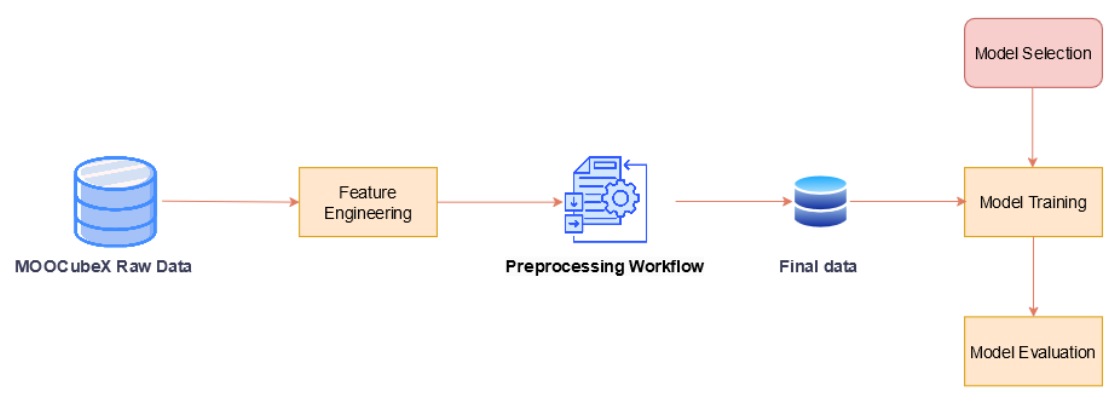
\includegraphics[width=0.75\linewidth]{figures/80.png}
    \caption{Framework tổ chức dữ liệu thực nghiệm}
\end{figure}
\label{sec:chuanbidulieu}
\subsubsection{Dịch bảng}
Trong quá trình chuyển ngữ từ Trung sang Tiếng Anh, chúng em đã tận dụng thư viện "googletrans" - một công cụ Python không mất phí và không giới hạn số lần dịch. Thư viện này vận hành thông qua API Google Translate Ajax để thực hiện các tác vụ như nhận diện ngôn ngữ và dịch thuật.\\
\\
Do khối lượng dữ liệu lớn, quá trình dịch gặp phải một số thách thức về thời gian và kết nối. Để khắc phục, chúng em đã triển khai các giải pháp sau:
\begin{quote}
\begin{itemize}
    \item Lưu lại tiến trình dịch để tránh mất dữ liệu
    \item Thiết lập cơ chế tự động gửi lại yêu cầu khi mất kết nối
    \item Ứng dụng thư viện "asyncio" cho phép gửi đồng thời nhiều API, giúp tối ưu tốc độ xử lý
\end{itemize}
\end{quote}
Đây là một phần code mẫu đã sử dụng phương pháp đã nêu trên:\\
\begin{figure}[H]
    \centering
    \includegraphics[width=0.75\linewidth]{figures/1.png}
\end{figure}
\newpage
Ngoài ra, chúng em nhận thấy không cần thiết phải dịch toàn bộ các trường dữ liệu lớn để huấn luyện mô hình vì một số trường dữ liệu không hỗ trợ cho việc huấn luyện mô hình. Thay vào đó, chúng em chỉ tập trung dịch 1 số trường sau đây:
\begin{quote}
-\textbf{course.json:} dịch cột “name”, “field”, “prerequisites” và “about”\\
\begin{figure}[H]
    \centering
    \includegraphics[width=0.75\linewidth]{figures/2.png}
\end{figure}
-\textbf{user.json:} dịch cột “school”
\begin{figure}[H]
    \centering
    \includegraphics[width=0.8\linewidth]{figures/3.png}
\end{figure}
\newpage
-\textbf{teacher.json:} Tiến hành dịch tất cả (trừ “id” và “name”)\\
\begin{figure}[H]
    \centering
    \includegraphics[width=1\linewidth]{figures/4.png}
\end{figure}
-\textbf{concept.json:} Dịch tất cả các cột của bảng này vì toàn bộ đều ở dạng chuỗi
\begin{figure}[H]
    \centering
    \includegraphics[width=1\linewidth]{figures/5.png}
\end{figure}
-\textbf{course-field.json:} Tiến hành dịch cột course\_name và field mang các thông tin dưới dạng chuỗi của bảng.
\begin{figure}[H]
    \centering
    \includegraphics[width=1\linewidth]{figures/6.png}
\end{figure}
\end{quote}
\subsubsection{Khám phá dữ liệu}
\textbf{a) Bảng course.json}
Ta xem qua bảng course.json:
\begin{figure}[H]
    \centering
    \includegraphics[width=1\linewidth]{figures/7.png}
\end{figure}
Ta xét độ dài của 3 cột “about”, “name\_trans” và “resource”:
\begin{figure}[H]
    \centering
    \includegraphics[width=0.485\linewidth]{figures/8.png}
\end{figure}
\newpage
Ta có thể thấy được 1 số thông tin từ dữ liệu trên:
\begin{itemize}
    \item Có những dòng dữ liệu không tồn tại cột “about”, tồn tại giá trị ngoại tệ ở cột “about” vì mean là 393 mà max lên đến 2293. Ta thể hiện trên boxplot độ dài của cột “about”:
    \begin{figure}[H]
        \centering
        \includegraphics[width=0.75\linewidth]{figures/9.png}
    \end{figure}
    \item Có thể thấy thật sự nhiều giá trị ngoại tệ cần được xử lí.
    \item Có những dòng dữ liệu không có resource\_length, mean cũng rất ngắn (71) chứng tỏ ít thông tin về khoá học.
\end{itemize}
Ta phân tích sâu cột “resource”:
\begin{figure}[H]
    \centering
    \includegraphics[width=0.75\linewidth]{figures/10.png}
\end{figure}
Mỗi resource trong bảng 2 là 1 tập hợp các video hay một tập các exercise. Mỗi resource sẽ có thêm 1 resource\_id là id của resource, chapter là chương chứa resource trong khóa học, titles gồm các tiêu đề như tiêu đề chương, video chương.\\
Thông tin của resource có thể tìm thấy trong file course.json. Một resource có 2 loại: Video và Exercise. Nếu loại tài nguyên là video, nó được xác định bằng ID video bắt đầu bằng ký tự V\_. Nhiều video\_id khác nhau tương ứng với một ccid, và ccid xác định duy nhất một video. Các video\_id này tương ứng với việc hiển thị cùng một video ccid tại các thời gian bắt đầu khác nhau. Mối liên hệ giữa video\_id và ccid được lưu trong relations/video\_id-ccid.txt. Phụ đề video có thể được tìm thấy trong tệp entities/video.json thông qua ccid.\\
Ta sẽ kiểm tra xem có bao nhiêu ID video không hợp lệ để phục vụ cho quá trình xử lý dữ liệu sau này:
\begin{figure}[H]
    \centering
    \includegraphics[width=0.75\linewidth]{figures/11.png}
\end{figure}
Có 2397 video ID không tồn tại, ta sẽ lọc đi hỗ trợ cho hiển thi thông tin trong tương lai.
Ta bắt đầu tiến hành đếm số khoá học trong cột “name\_trans”, chia bởi lĩnh vực (cột “field”):\\
\begin{figure}[H]
    \centering
    \includegraphics[width=0.35\linewidth]{./figures/12.png}
\end{figure}
\newpage
\begin{figure}[H]
    \centering
    \includegraphics[width=0.7\linewidth]{figures/13.png}
\end{figure}
Ta thấy có tổng 3781 khoá học và 81 lĩnh vực, với “computer science and technology” đứng đầu với 63 khoá học, chiếm 6.8\% trên tổng khoá học. Ta cũng kiểm tra với mỗi khoá học được xếp bao nhiêu lĩnh vực (cột “field”):
\begin{figure}[H]
    \centering
    \includegraphics[width=0.9\linewidth]{figures/14.png}
\end{figure}
Ta có thể thấy có rất nhiều khoá học không thuộc lĩnh vực nào, có rất nhiều khóa học không có field nào, có thể cột “field” sẽ không đóng góp nhiều trong xây dựng thuật toán hoặc cần xử lí.\\
\textbf{b) Bảng user.json}\\
Đầu tiên, ta đọc dữ liệu và quan sát dữ liệu thông qua dạng bảng (DataFrame):
\begin{figure}[H]
    \centering
    \includegraphics[width=1\linewidth]{figures/15.png}
\end{figure}
\newpage
Ta tiến hành thống kê đặc điểm từng cột có trong bảng:
\begin{figure}[H]
    \centering
    \includegraphics[width=1\linewidth]{figures/16.png}
    \caption{Số lượng users}
\end{figure}
\begin{figure}[H]
    \centering
    \includegraphics[width=1\linewidth]{figures/17.png}
    \caption{Cột “gender”}
\end{figure}
\begin{figure}[H]
    \centering
    \includegraphics[width=1\linewidth]{figures/18.png}
    \caption{Phân bố các các giá trị trong cột “gender”:}
\end{figure}
\newpage
\begin{figure}[H]
    \centering
    \includegraphics[width=1\linewidth]{figures/19.png}
    \caption{Thông tin cột “school”}
\end{figure}
\begin{figure}[H]
    \centering
    \includegraphics[width=1\linewidth]{figures/20.png}
    \caption{Số lượng trường học trong bảng}
\end{figure}
\begin{figure}[H]
    \centering
    \includegraphics[width=1\linewidth]{figures/21.png}
    \caption{Kiểm tra thông tin tổng quan sau cùng}
\end{figure}
\newpage
\begin{figure}[H]
    \centering
    \includegraphics[width=1\linewidth]{figures/22.png}
    \caption{Số lượng sample (users) có trong bảng và số lượng users thuộc về mỗi trường học}
\end{figure}
\begin{figure}[H]
    \centering
    \includegraphics[width=1\linewidth]{figures/23.png}
    \caption{Tạo một cột “school\_length” để phân tích độ dài mỗi sample của cột}
\end{figure}
\newpage
\begin{figure}[H]
    \centering
    \includegraphics[width=0.68\linewidth]{figures/24.png}
    \caption{Trực quan hóa độ dài của sample cột “school”}
\end{figure}
\begin{figure}[H]
    \centering
    \includegraphics[width=0.68\linewidth]{figures/25.png}
    \caption{Trực quan hóa phân bố các giá trị của cột “gender”}
\end{figure}
\newpage
\textbf{c) Bảng teacher.json}\\
Sau đây là các thống số cơ bản của bảng
\begin{figure}[H]
    \centering
    \includegraphics[width=0.6\linewidth]{figures/27.png}
\end{figure}
Tham khảo phân phối của top 10 tên việc xuất hiện nhiều nhất trong bảng
\begin{figure}[H]
    \centering
    \includegraphics[width=0.75\linewidth]{figures/28.png}
\end{figure}
Tham khảo phân phối của top 10 tổ chức xuất hiện nhiều nhất trong bảng
\newpage
\begin{figure}[H]
    \centering
    \includegraphics[width=0.75\linewidth]{figures/29.png}
\end{figure}
Ta thực hiện phân tích mối quan hệ giữa ba chức vụ (job titles) có số lượng giáo viên nhiều nhất và mười tổ chức (organizations) có số lượng giáo viên cao nhất
\begin{figure}[H]
    \centering
    \includegraphics[width=0.95\linewidth]{figures/30.png}
\end{figure}
\newpage
\begin{figure}[H]
    \centering
    \includegraphics[width=0.65\linewidth]{figures/31.png}
\end{figure}
Sau khi lọc bỏ các liên kết có khóa học hoặc teacher không tồn tại dựa vào file course-teacher.txt, số hàng còn lại là 35593. Các thông tin được trực quan hóa như sau
\begin{figure}[H]
    \centering
    \includegraphics[width=0.8\linewidth]{figures/32.png}
    \caption{Histogram thể hiện số lượng khóa học của mỗi teacher và bảng thống kê mô tả tương ứng}
\end{figure}
\newpage
\begin{figure}[H]
    \centering
    \includegraphics[width=0.8\linewidth]{figures/33.png}
    \caption{Histogram thể hiện số lượng teacher của mỗi khóa học và bảng thống kê mô tả tương ứng}
\end{figure}
\textbf{d) Bảng school.json}
Ta đếm dữ liệu ở từng cột, đếm các giá trị đặc biệt, giá trị xuất hiện nhiều nhất với tần số của nó:
\begin{figure}[H]
    \centering
    \includegraphics[width=0.75\linewidth]{figures/34.png}
\end{figure}
Kiểm tra kiểu dữ liệu của từng cột: 
\newpage
\begin{figure}[H]
    \centering
    \includegraphics[width=0.6\linewidth]{figures/35.png}
\end{figure}
Ta tạo 2 cột mới là “about\_length” và “motto\_length” để lần lượt thể hiện độ dài của giá trị dữ liệu ở 2 cột “about” và “motto”:
\begin{figure}[H]
    \centering
    \includegraphics[width=0.65\linewidth]{figures/36.png}
\end{figure}
\newpage
Có 2 cột ta cần là “about\_length” và “motto\_length” để ta tìm phân bố độ dài của giá trị lên đồ thị:
\begin{figure}[H]
    \centering
    \includegraphics[width=0.7\linewidth]{figures/37.png}
\end{figure}
Dựa vào biểu đồ ta có thể nhận xét rằng mô tả của các trường đều rất chi tiết, số lượng trường với số lượng từ phần mô tả > 2000  chiếm phần lớn. Tuy nhiên thông tin này có vẻ không hữu ích với hệ thống khuyến nghị.
\begin{figure}[H]
    \centering
    \includegraphics[width=0.7\linewidth]{figures/38.png}
\end{figure}
Hầu hết các trường đại học đều có một khẩu hiệu ngắn gọn dưới 20 từ vì chủ yếu khẩu hiệu sẽ đơn giản nhất có thể để truyền đạt tầm nhìn và mục tiêu của trường một cách trực tiếp ngắn gọn, đọng lại trong trí nhớ người xem. Một phần nhỏ hơn các trường có khẩu hiệu tương đối dài với 40 đến 88 chữ. 
\newpage
\textbf{e) Bảng course-field.json}
\begin{figure}[H]
    \centering
    \includegraphics[width=1\linewidth]{figures/39.png}
    \caption{Tổng số lượng khóa học và tổng số lượng các lĩnh vực khác nhau}
\end{figure}
\begin{figure}[H]
    \centering
    \includegraphics[width=1\linewidth]{figures/40.png}
    \caption{Phân bố số lượng khóa học theo từng lĩnh vực}
\end{figure}
\newpage
\begin{figure}[H]
    \centering
    \includegraphics[width=0.85\linewidth]{figures/41.png}
    \caption{Phân bố độ dài tên khóa học}
\end{figure}
\begin{figure}[H]
    \centering
    \includegraphics[width=0.9\linewidth]{figures/42.png}
    \caption{Biểu đồ thanh thể hiện sự phân bố số lượng khóa học theo từng lĩnh vực}
\end{figure}
\newpage
\begin{figure}[H]
    \centering
    \includegraphics[width=0.75\linewidth]{figures/44.png}
    \caption{Biểu đồ phân phối cho độ dài tên khóa học}
\end{figure}
\subsubsection{Làm sạch dữ liệu}
\textbf{a) Bảng course.json}\\
Ta kiểm tra dữ liệu thiếu, dữ liệu không nhất quán, dữ liệu trùng lặp và dữ liệu trống:
\\
Đầu tiên ta thấy được có 647 giá trị ở cột “name\_trans” bị trùng lặp cho dù id không bị trùng, chứng tỏ có sự lỗi nhất định trong bộ dữ liệu, cũng như nãy đã thống kê ta thấy được có rất nhiều giá trị trống ở cột “field\_trans”.\\
\\
Ta kiểm tra kĩ hơn về các dòng có giá trị trong cột “name” bị trùng lặp:
\begin{figure}[H]
    \centering
    \includegraphics[width=1\linewidth]{figures/26.png}
\end{figure}
\newpage
\begin{figure}[H]
    \centering
    \includegraphics[width=1\linewidth]{figures/45.png}
\end{figure}
Ta thấy được đa số dữ liệu trong này cột “field” đa số bị trống và trùng lặp, cũng như các cột khác không có ý nghĩa hoặc trùng với các cột khác, thực hiện chi square test, ta có được kết quả với P-value rất thấp, chứng tỏ các giá trị phụ thuộc với nhau chứ không hề có giá trị mới. Chứng tỏ ta có thể xoá được các dòng dữ liệu này, cũng như các khoá học không tồn tại trong “course-field.json”.\\
\textbf{b) Bảng user.json}\\
Ta thấy cột “year\_of\_birth” bị thiếu dữ liệu hơn 97\% trong khi các cột còn lại tỉ lệ \% thiếu là rất thấp. Ta tiến hành loại bỏ cột này, sau đó ta sẽ tiến hành xử lý dữ liệu nhiễu trên cột gender với 2 giá trị nhiễu là 232 và 3\\
\textbf{c) Bảng concept.json}\\
Ta thấy cột “id” bị thiếu 207 giá trị, ta tiến hành bỏ các hàng này.\\
\begin{figure}[H]
    \centering
    \includegraphics[width=1\linewidth]{figures/46.png}
\end{figure}
\newpage
Ta kiểm tra kĩ hơn về các bản ghi có giá trị trùng lặp và xử lý chúng:\\
\begin{figure}[H]
    \centering
    \includegraphics[width=1\linewidth]{figures/47.png}
\end{figure}
\textbf{d) Bảng course-field.json}\\
Sử dụng isnull().sum() để tính số lượng giá trị thiếu trong từng cột. Sau đó loại bỏ hàng chứa giá trị thiếu bằng cách sử dụng dropna()
\newpage
\begin{figure}[H]
    \centering
    \includegraphics[width=1\linewidth]{figures/48.png}
\end{figure}
Dữ liệu văn bản thường chứa nhiều thông tin nhiễu chẳng hạn như các ký tự không mong muốn: Các ký tự đặc biệt, dấu câu, hoặc ký tự không phải chữ cái có thể làm giảm chất lượng phân tích. Ở đây chúng ta sẽ tiến hành loại bỏ các ký tự không cần thiết, các khoảng trắng dư thừa và thường hóa các ký tự viết hoa\\
\\
Để kiếm tra dữ liệu trùng lặp, chúng ta sử dụng phương thức duplicated() trong pandas. Đầu tiên xác định các bản ghi trùng lặp, sau đó đếm số lượng và hiển thị các bảng ghi trùng lặp đó. Sau đó tiến hành xóa bản ghi trùng lặp bằng cách sử dụng drop\_duplicates()
\newpage
\begin{figure}[H]
    \centering
    \includegraphics[width=1\linewidth]{figures/49.png}
\end{figure}
\textbf{e) Bảng school.json}\\
Ta xoá cột “name” đi vì trùng với ý nghĩa với cột “name\_en” (tên nhưng trong Tiếng Anh)\\
\\
Ta thống nhất cột “sign” (kí hiệu đại diện cho trường) đều là tất cả in hoa:
\newpage
\begin{figure}[H]
    \centering
    \includegraphics[width=0.7\linewidth]{figures/50.png}
\end{figure}
Vì ở đây tên trường (“name\_en”) cũng như kí hiệu (“sign”) là chìa khoá chính, hay nói cách khác là giá trị duy nhất nên không thể có dòng trùng với nhau, ta tiến hành xoá các dòng trùng giá trị:
\begin{figure}[H]
    \centering
    \includegraphics[width=0.7\linewidth]{figures/51.png}
\end{figure}
\textbf{g) Bảng teacher.json}\\
Ở đây có cột name\_en bị thiếu nên điền vào cột đó bằng cách lấy phiên âm của cột name là được. Để làm việc này có thể sử dụng thư viện pypinyin để lấy phát âm dùng cho tên tiếng anh.
\clearpage
\begin{figure}[H]
    \centering
    \includegraphics[width=0.7\linewidth]{figures/52.png}
\end{figure}

\subsubsection{Chuyển đổi dữ liệu}
\textbf{Feature Engineering:}
Nhóm sẽ chọn các bảng và thuộc tính có thể sử dụng để tạo ra feature các mô hình khuyến nghị dựa trên bộ dữ liệu đã xử lý và làm sạch trước đó:\\
\\
Các bảng được chọn và thuộc tính sử dụng:
\begin{figure}[H]
    \centering
    \includegraphics[width=0.6\linewidth]{figures/53.png}
\end{figure}
\newpage
\begin{itemize}
    \item Với ‘user.json’: ‘course\_order’ gồm các khóa học mà user đã đăng ký với khóa học sau cùng là khóa học gần đây nhất, dùng để tạo liên kết giữa ‘user.json’ và ‘course.json’.
    \item Với ‘course.json’: Đây là table quan trọng chứa thông tin về các khóa học như ‘name’, ‘about’ và ‘field’.
    \item Với ‘teacher.json’, ‘school.json’: dùng để tạo relation với ‘course.json’ chứa thông tin về trường tổ chức khóa học và giáo viên giảng dạy.
    \item Với ‘course-field.json’: chứa các field của mỗi khóa học, dùng để kiểm tra với trường ‘field’ trong ‘course.json’.
    \item Với ‘concept.json’: id theo quy ước ‘K\_{concept name}{field}’, tạo thêm feature concept-name\_field với mỗi khoá học.
\end{itemize}
Tạo knowledge graph:
\begin{figure}[H]
    \centering
    \includegraphics[width=0.3\linewidth]{figures/54.png}
\end{figure}
Tạo interaction giữa người dùng với khóa học: sử dụng 5-core filtering, lọc người dùng với ít hơn 5 khóa học và những khóa học có số lượng đăng ký dưới 5.\\
Kết quả: Vì data đã được xử lý trước đó nên ta thấy không có thay đổi đáng kể
\begin{center}
\begin{tabular}{|| m{15em}  m{15em}||} 
 \hline
 Trước khi filter & Sau khi filter\\ [0.5ex] 
 \hline\hline
 1.183.774 interactions & 1.182.745 interactions \\ [1ex]
 \hline
\end{tabular}
\end{center}
\newpage
Tạo relation giữa các entities: course-relation-attribute. Sau đó ta tiến hành lọc theo tiêu chí, số lần course xuất hiện tối thiểu là 5 và số lần xuất hiện tối thiểu của một relation là 25. \\
Kết quả: 
\begin{center}
\begin{tabular}{|| m{15em}  m{15em}||} 
 \hline
 Trước khi filter & Sau khi filter\\ [0.5ex] 
 \hline\hline
 376.093 interactions & 71.787 interactions \\ [1ex]
 \hline
\end{tabular}
\end{center}
\subsubsection{Chia tập dữ liệu}
\begin{itemize}
    \item Dữ liệu cuối cùng được chia theo chiến lược leave-one-out: Với mỗi user, nhóm giữ khoá học cuối cùng làm test, các khoá học còn lại làm train. 
    \item Dữ liệu cuối cùng để thực nghiệm có 4 loại dữ liệu chính: dữ liệu thô (chưa xử lí), 10\% dữ liệu thô, dữ liệu đã xử lí (chiến lược leave-one-out) và 10\% dữ liệu đã xử lí.
\end{itemize}

\subsection{Độ đo đánh giá}
Để đánh giá performance của mô hình, nhóm sử dụng cách đánh giá \textit{leave-one-out}. Các mô hình được đánh giá theo chiến lược “randomly sampling negative item”, nghĩa là bắt cặp khóa học ground truth trong tập test với 100 khóa học mà người dùng chưa đăng ký được lấy mẫu ngẫu nhiên.

Về độ đo đánh giá, chúng tôi sử dụng 2 độ đo đánh giá phổ biến: \textit{Recall} và \textit{NDCG}.

\textbf{Recall:} \\
\textbf{Khái niệm:} Recall đo lường mức độ mà hệ thống khuyến nghị có thể đề xuất các khóa học liên quan đến người dùng trong tất cả các khóa học phù hợp mà họ quan tâm. \\
\textbf{Ý nghĩa:} Giá trị Recall cao nghĩa là hệ thống khuyến nghị không bỏ sót quá nhiều khóa học phù hợp với người dùng. Ví dụ, nếu hệ thống đề xuất được tất cả các khóa học mà người dùng có thể quan tâm, Recall sẽ đạt giá trị tối đa là 1 (100\%). \\

\textbf{Công thức:}
\[
\text{Recall@K} = \frac{\text{Số lượng khóa học phù hợp trong top K}}{\text{Tổng số khóa học phù hợp có trong hệ thống}}
\]

\textbf{Ví dụ:} Giả sử một người dùng có 20 khóa học trong hệ thống mà họ thực sự quan tâm, và hệ thống đề xuất 10 khóa học, trong đó có 5 khóa học phù hợp. Khi đó:
\[
\text{Recall@10} = \frac{5}{20} = 0.25
\]
Điều này có nghĩa là hệ thống đã thu hút được 25\% các khóa học liên quan cho người dùng trong số những gì họ có thể quan tâm. Tỷ lệ này càng cao, khả năng đáp ứng nhu cầu của hệ thống càng tốt.

\textbf{NDCG (Normalized Discounted Cumulative Gain):} \\
\textbf{Khái niệm:} NDCG đánh giá chất lượng của xếp hạng các khóa học được đề xuất, nhấn mạnh sự ưu tiên của các khóa học ở các vị trí đầu tiên trong danh sách. \\
\textbf{Ý nghĩa:} Một xếp hạng lý tưởng (perfect ranking) là khi các khóa học phù hợp nhất nằm ở đầu danh sách. NDCG giúp đánh giá mức độ chính xác của hệ thống khi xếp hạng những khóa học này. Giá trị NDCG nằm trong khoảng từ 0 đến 1, với 1 là lý tưởng nhất, nghĩa là thứ tự của các khóa học được hệ thống xếp đúng như thứ tự mà người dùng mong muốn. \\

\textbf{Công thức:}
\[
\text{NDCG@K} = \frac{\text{DCG@K}}{\text{IDCG@K}}
\]
\textbf{DCG@K (Discounted Cumulative Gain):} Đánh giá mức độ liên quan của các khóa học theo thứ tự xếp hạng nhưng giảm dần theo logarit của vị trí:
\[
\text{DCG@K} = \sum_{i=1}^{K} \frac{\text{rel}_i}{\log_2(i+1)}
\]
Trong đó $\text{rel}_i$ là độ liên quan (relevance score) của khóa học ở vị trí $i$. Giá trị $\text{rel}_i$ thường được cho là 1 nếu khóa học phù hợp, và 0 nếu không. \\

\textbf{IDCG@K (Ideal DCG):} Là giá trị DCG trong trường hợp xếp hạng lý tưởng nhất, tức là khi các khóa học liên quan nhất được xếp lên đầu tiên.

\textbf{Ví dụ:} Giả sử hệ thống đề xuất 3 khóa học và người dùng quan tâm nhiều nhất đến khóa học thứ nhất và thứ ba: \\
Nếu thứ tự thực tế của hệ thống là [khóa học 1, khóa học 2, khóa học 3], DCG sẽ là:
\[
\text{DCG@3} = 1 + 0 + \frac{1}{\log_2(3+1)} = 1 + 0 + 0.5 = 1.5
\]
Nếu thứ tự lý tưởng là [khóa học 1, khóa học 3, khóa học 2], IDCG sẽ là:
\[
\text{IDCG@3} = 1 + \frac{1}{\log_2(2+1)} + 0 = 1 + 0.63 + 0 = 1.63
\]
Khi đó:
\[
\text{NDCG@3} = \frac{\text{DCG@3}}{\text{IDCG@3}} = \frac{1.5}{1.63} \approx 0.92
\]
Giá trị 0.92 cho thấy hệ thống xếp hạng gần như lý tưởng nhưng vẫn có một sai lệch nhỏ.




\subsection{Kịch bản thực nghiệm}
Nhóm sẽ chia bộ dữ liệu thành 4 loại Dataset, mỗi Dataset được chia theo phương pháp leave-one-out như đề cập ở trên. Đây cũng chính là kich bản thực nghiệm theo thời gian trên kiến trúc dữ liệu lớn. Sau khi huấn luyện các mô hình, nhóm sẽ đánh giá trên tập test.
\paragraph{Thông số chi tiết của các phương pháp}
\subsubsection{Content-based filtering}
\textbf{}\\
\textbf{Feature 1:} 
\begin{itemize}
    \item Sử dụng trường name, about, field của khóa học.
    \item TFIDF để chuyển thông tin thành vector
    \item Tính độ tương đồng giữa khóa học và người dùng bằng cosine
\end{itemize}
\textbf{Feature 2:}
\begin{itemize}
    \item Sử dụng school, concept của khóa học
    \item TFIDF để chuyển thông tin thành vector
    \item Tính độ tương đồng giữa khóa học và người dùng bằng cosine
\end{itemize}
\textbf{Feature 3:} 
\begin{itemize}
    \item Sử dụng school, concept của khóa học
    \item Multi-hot encoding để chuyển thông tin thành vector
    \item Tính độ tương đồng giữa khóa học và người dùng bằng cosine
\end{itemize}
\subsubsection{Matrix factorization (MF)}
\begin{itemize}
    \item Course embedding dimension = User embedding dimension = 64
    \item Lambda của l2 regularization = 10$^{-5}$
    \item Train batch size =  1024
    \item Test batch size = 10000
    \item Optimizer: Adam
    \item Learning rate = 0.0001
    \item Số epoch = 300
    \item Evaluate every 5 epochs Early stopping steps = 5 với Recall@10→ Thực nghiệm dừng tại epoch 140
\end{itemize}
\subsubsection{Factorization machine}
\begin{itemize}
    \item Course embedding dimension = User embedding dimension = 64
    \item Lambda của l2 regularization = 10$^{-5}$
    \item Train batch size = Test batch size = 1024
    \item Optimizer: Adam
    \item Learning rate = 0.0001
    \item Số epoch = 1000
    \item Evaluate every 5 epochs Early stopping steps = 10 với Recall@10
\end{itemize}
\subsubsection{Neural Factorization Machine}
\begin{itemize}
    \item Course embedding dimension = User embedding dimension = 64
    \item Gồm 3 hidden layers nối tiếp nhau, mỗi hidden layer là một linear layer với activation là ReLU, được theo sau bởi 1 lớp dropout với dropout rate là 0.1.
    \item Ba hidden layers có output dimension lần lượt là 64, 32, 16.
    \item Lambda của l2 regularization = 10$^{-5}$
    \item Train batch size = Test batch size = 1024
    \item Optimizer: Adam Learning rate = 0.0001
    \item Số epoch = 1000
    \item Evaluate every 5 epochs
    \item Early stopping steps = 5 với Recall@10
\end{itemize}
\subsubsection{Knowledge Graph Attention Network (KGAT)}
\begin{itemize}
    \item Course embedding dimension = User embedding dimension = Relation embedding dimension = 64
    \item Train batch size:
    \begin{itemize}
        \item Collaborative batch size = 1024
        \item Knowledge graph batch size = 2048
    \end{itemize}
    \item Test batch size = 256
    \item Laplacian type: random walk
    \item Aggregation type: bi-interaction
    \item Độ sâu là 3 với hidden dimension là 64, 32, 16.
    \item Lambda của knowledge graph’s l2 regularization = 10$^{-5}$
    \item Lambda của collaborative’s l2 regularization = 10$^{-5}$
    \item Optimizer: Adam
    \item Learning rate = 0.0001
    \item Số epoch = 1000
    \item Evaluate every 5 epochs Early stopping steps = 10 với Recall@10
\end{itemize}
\subsection{Đánh giá kết quả thực nghiệm}
\textbf{}\\
\label{sec:ketqua}
\begin{figure}[h]
    \centering
    \includegraphics[width=0.8\textwidth]{figures/71.png}
    \caption{Bảng kết quả thực nghiệm}
\end{figure}
\begin{figure}
    \centering
    \includegraphics[width=1\linewidth]{figures/recall.png}
    \caption{Reall@K của 5 thực nghiệm}
\end{figure}
\begin{figure}
    \centering
    \includegraphics[width=1\linewidth]{figures/ndcg.png}
    \caption{NDCG@K của 5 thực nghiệm}
\end{figure}
\begin{figure}
    \centering
    \includegraphics[width=1\linewidth]{figures/recall_epoch.png}
\end{figure}
\begin{figure}
    \centering
    \includegraphics[width=1\linewidth]{figures/ndcg_epoch.png}
\end{figure}
\newpage
Dựa trên các kết quả đã biểu diễn, ta có thể nhận xét về ảnh hưởng của chất lượng dữ liệu đến hiệu quả của các model như sau:\\
\textbf{Sự cải thiện từ 10\% Raw sang 10\% Data:}
\begin{itemize}
    \item Với tất cả các model, việc sử dụng dữ liệu đã được xử lý (10\% Data) thay vì dữ liệu thô (10\% Raw) đều dẫn đến sự cải thiện đáng kể cả về Recall@10 và NDCG@10.
    \item Các model phức tạp như KGAT và NFM có mức tăng lớn hơn, do chúng có khả năng tận dụng tốt hơn các đặc trưng ẩn trong dữ liệu đã được xử lý. Điều này cho thấy rằng dữ liệu thô không đủ thông tin để các model này phát huy hiệu quả.
\end{itemize}
\textbf{Sự cải thiện từ 10\% Data lên 100\% Data:}
\begin{itemize}
    \item Khi tăng dung lượng và chất lượng dữ liệu từ 10\% lên 100\%, các model đều cho thấy sự cải thiện tiếp theo, nhưng mức tăng không đồng đều.
    \item Đặc biệt, các model như MF và KGAT đạt được hiệu quả tối ưu hơn nhờ khả năng xử lý lượng lớn dữ liệu và khai thác các mối quan hệ sâu sắc. Trong khi đó, các model đơn giản hơn như CBF có sự cải thiện ít hơn, do hạn chế về khả năng học đặc trưng phức tạp.
\end{itemize}
\textbf{Tương quan giữa chất lượng dữ liệu và phức tạp của model:}
\begin{itemize}
    \item Các model phức tạp hơn (như KGAT, NFM) phụ thuộc nhiều vào chất lượng dữ liệu. Khi dữ liệu được làm sạch và tăng dung lượng, hiệu quả của chúng cải thiện vượt trội hơn so với các model đơn giản (CBF).
    \item Điều này cho thấy rằng dữ liệu chất lượng cao không chỉ cải thiện hiệu quả tổng thể mà còn giúp khai thác tối đa tiềm năng của các model tiên tiến.
\end{itemize}
